\documentclass[conference]{IEEEtran}

\usepackage[T1]{fontenc}
\usepackage{lmodern}
\usepackage{amsmath,amssymb}
\usepackage{booktabs}
\usepackage{tabularx}
\usepackage{array}
\usepackage{url}
\usepackage{hyperref}
\usepackage{tikz}
\usetikzlibrary{arrows.meta,positioning,shapes.geometric}

\hypersetup{colorlinks=true,linkcolor=blue,citecolor=blue,urlcolor=blue}
\newcolumntype{Y}{>{\raggedright\arraybackslash}X}
\newcommand{\tool}{N-Day Nexus}

\begin{document}

\title{N-Day Nexus: Multi-Evidence Patch Assurance for Vulnerable Software}

\author{
\IEEEauthorblockN{%
\begin{tabular}{@{}*{3}{>{\centering\arraybackslash}p{0.31\textwidth}}@{}}
Nipun Nitin Bhattad & Krish Rohilla & Amitanshu Yadav \\[0.1em]
{\small Roll No.: 16} & {\small Roll No.: 25} & {\small Roll No.: 50} \\
{\footnotesize simplynb14@gmail.com} &
{\footnotesize krish4work25@gmail.com} &
{\footnotesize amitanshuyadav55@gmail.com}
\end{tabular}} \\[0.2em]
\IEEEauthorblockA{%
B.Tech, 5th Semester, [Section]\\
[Department], [Institution]\\
Information Security Lab, Course Code: [Course Code]\\
Faculty / Guide: [Faculty Name]\\
Academic Year: [Academic Year]}
}

\maketitle

\begin{abstract}
Security teams need practical evidence that a software update addresses a known vulnerability before adopting it across production systems. This paper presents \tool, a local patch-assurance workflow that compares vulnerable and fixed builds using controlled runtime probes, AddressSanitizer, source-patch inspection, and target-appropriate compiled-binary analysis. Five case studies cover memory corruption in sudo, CPython, and EditorConfig; AES-GCM parameter handling in OpenSSL; and out-of-memory request-state corruption in PHP. Each case uses a Docker-based vulnerable/patched pair and repeated target-specific probes. Four targets use Ghidra, BinExport, and BinDiff; PHP uses a six-file source comparison and ELF symbol analysis, which identify 1,093 changed source lines, 97 added symbols, and nine removed symbols. Its benign command probe recorded 0/5 command confirmations in the vulnerable build and 5/5 no-command outcomes in the patched build. The workflow combines traceable source, runtime, sanitizer, and binary evidence to help maintainers assess confidentiality, integrity, and availability properties during release review.
\end{abstract}

\begin{IEEEkeywords}
software security, patch assurance, vulnerability analysis, binary diffing, memory safety
\end{IEEEkeywords}

\section{Introduction}
\subsection{Background}
Software vulnerabilities can affect confidentiality, integrity, and availability (CIA). A memory-safety defect can corrupt program state or terminate a process; a cryptographic API defect can weaken protection of encrypted data. Security updates change source code and compiled behavior, and operators need a repeatable way to evaluate those changes against their deployment requirements. NIST's Secure Software Development Framework (SSDF) recommends integrating security practices into development and vulnerability response activities \cite{nistssdf}.

\tool{} is designed as a local patch-assurance workflow. It builds vulnerable and patched versions of selected open-source components, applies controlled probes to both versions, compares their source and compiled binaries, and presents the evidence in a report and dashboard. Its defensive purpose is to help a maintainer assess the behavior of a selected update before using that update as a release or remediation decision.

\subsection{Problem Statement}
Patch review often requires reading source changes, reproducing a security issue, and understanding how a compiled binary changed. These tasks are performed with different tools and can be difficult to connect into one reviewable result. The project addresses this by joining source-level patch evidence, runtime observations, sanitizer diagnostics, and function-level binary comparison in one paired experiment.

\subsection{Research Gap}
Source review explains intended code changes, runtime testing observes behavior for specific inputs, sanitizers identify instrumented memory errors, and binary diff tools help locate changed functions. Each evidence type answers a different question. The project combines these techniques around a controlled vulnerable-versus-patched comparison and maps target findings to CIA objectives, supporting a practical release-assurance workflow.

\subsection{Objectives}
The project objectives are:
\begin{itemize}
  \item Build pinned vulnerable and patched versions with reproducible Docker definitions.
  \item Apply equivalent, safe, target-specific probes to both builds and record repeated outcomes.
  \item Collect AddressSanitizer evidence for memory-safety cases.
  \item Apply target-appropriate compiled-binary analysis: Ghidra, BinExport, and BinDiff, or ELF symbol comparison.
  \item Present source, runtime, and binary evidence in a dashboard and machine-readable report.
  \item Support defensive patch decisions by relating each case to confidentiality, integrity, or availability.
\end{itemize}

\subsection{Paper Organization}
Section II reviews related security-assurance tools and practices. Section III describes the architecture, target cases, probe preparation, and evaluation. Section IV summarizes the artifact inventory and the CIA-oriented interpretation. Section V concludes and lists future extensions.

\section{Related Work}
The NIST SSDF provides a framework for incorporating secure development and vulnerability response practices into software lifecycles \cite{nistssdf}. NIST's software verification guidance places testing and verification within a broader assurance process \cite{nistverify}. \tool{} applies this perspective to patch assessment by retaining evidence that can be inspected during dependency updates and release reviews.

Ghidra is an extensible software reverse-engineering framework that supports disassembly, decompilation, scripting, and binary analysis \cite{ghidra}. BinDiff compares disassembled programs through function and control-flow graph matching; its similarity and confidence values help prioritize review \cite{bindiff}. In this project, Ghidra prepares binary analysis and function evidence, BinExport transfers the analysis representation, and BinDiff matches functions across the version pair.

AddressSanitizer (ASan) instruments programs to detect out-of-bounds accesses, use-after-free conditions, and related memory errors during execution \cite{asan}. Its diagnostics complement ordinary process outcomes by identifying invalid memory accesses in instrumented builds. Runtime probes add target-specific observations, while source-patch review connects those observations with the change introduced by the maintainer.

\tool{} combines these established methods as a paired experimental workflow. Its contribution is the integration of build, probe, sanitizer, source-diff, and binary-diff artifacts with an operator-oriented report, allowing reviewers to trace a security decision from the target versions to observed evidence.

\section{Methodology}
\subsection{System Architecture}
Fig.~\ref{fig:architecture} summarizes the pipeline. Target metadata specifies the component, version pair, affected source location, binary path, build definitions, and probe mode. The builder creates two isolated images. Runtime validation executes the configured probe in each image. Patch analysis follows the target's configured path: Ghidra, BinExport, and BinDiff for four cases, and source plus ELF-symbol comparison for PHP. The reporter combines the findings and the dashboard organizes the results for review.

\begin{figure*}[t]
\centering
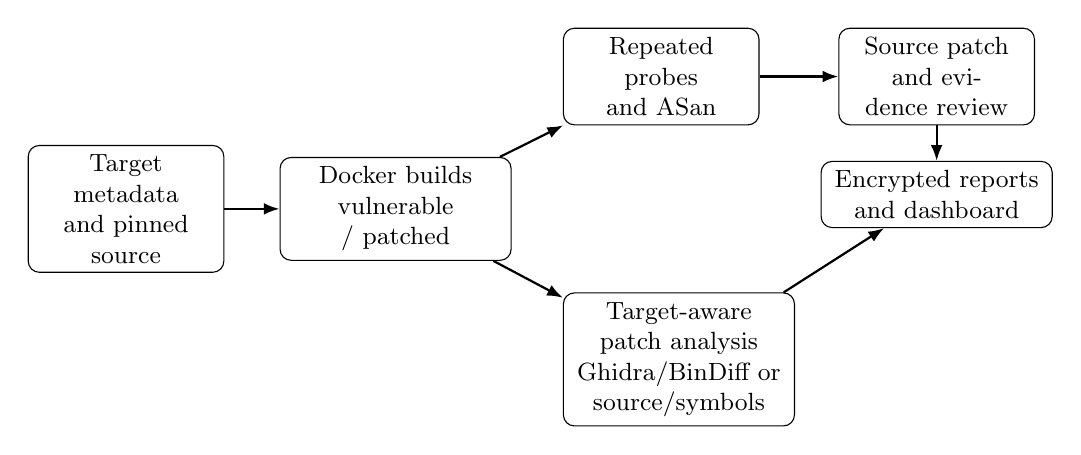
\begin{tikzpicture}[
  node distance=0.55cm and 0.7cm,
  box/.style={draw,rounded corners,align=center,minimum height=0.8cm,text width=2.25cm,font=\small},
  wide/.style={draw,rounded corners,align=center,minimum height=0.8cm,text width=2.7cm,font=\small},
  arr/.style={-{Latex[length=2mm]},thick}
]
\node[box] (config) {Target metadata\\and pinned source};
\node[wide,right=of config] (build) {Docker builds\\vulnerable / patched};
\node[box,above right=0.4cm and 0.65cm of build] (runtime) {Repeated probes\\and ASan};
\node[wide,below right=0.4cm and 0.65cm of build] (reverse) {Target-aware patch analysis\\Ghidra/BinDiff or source/symbols};
\node[box,right=1.0cm of runtime] (evidence) {Source patch\\and evidence review};
\node[wide,below=0.45cm of evidence] (report) {Encrypted reports\\and dashboard};
\draw[arr] (config) -- (build);
\draw[arr] (build) -- (runtime);
\draw[arr] (build) -- (reverse);
\draw[arr] (runtime) -- (evidence);
\draw[arr] (reverse) -- (report);
\draw[arr] (evidence) -- (report);
\end{tikzpicture}
\caption{N-Day Nexus paired-build patch-assurance pipeline.}
\label{fig:architecture}
\end{figure*}

\subsection{Dataset}
The evaluation set contains five historical vulnerability cases selected to exercise different patch-validation evidence paths. Four cases involve memory corruption or request-state corruption; one focuses on a cryptographic API parameter-handling defect. Table~\ref{tab:targets} gives the configured versions and security property associated with each case. Version identifiers and source locations come from the target metadata and upstream project references \cite{sudoCVE,pythonCVE,editorCVE,opensslCVE,phpCVE}.

\begin{table*}[t]
\caption{Configured Vulnerability Cases}
\label{tab:targets}
\centering
\small
\begin{tabularx}{\textwidth}{@{}l l l Y Y@{}}
\toprule
\textbf{CVE} & \textbf{Component} & \textbf{Version pair} & \textbf{Patch focus} & \textbf{CIA review objective} \\
\midrule
CVE-2019-18634 & sudo & 1.8.25p1 / 1.8.31p1 & Password-input pointer/capacity handling in \texttt{tgetpass} & Integrity of process memory; availability under crafted input \\
CVE-2021-3177 & CPython \texttt{ctypes} & 3.9.1 / 3.9.2 & Large floating-point formatting in \texttt{PyCArg\_repr} & Integrity of memory and continued process availability \\
CVE-2023-0341 & editorconfig-core-c & 0.12.5 / 0.12.6 & Capacity checks while constructing the \texttt{ec\_glob} pattern & Integrity of stack state; availability during parsing \\
CVE-2023-5363 & OpenSSL EVP & 3.0.11 / 3.0.12 & Ordering of AEAD key-length and IV-length parameters & Confidentiality of AES-GCM protected data \\
CVE-2026-109618 & PHP Apache mod\_php & 8.4.26 / 8.4.27 & OOM recovery and request-state cleanup & Confidentiality, integrity, and availability under RCE impact \\
\bottomrule
\end{tabularx}
\end{table*}

\subsection{Preprocessing}
Build inputs are pinned to upstream tags or commits in each target's Dockerfiles and metadata. Both versions use their target-specific build configuration. The probe uses the configured binary path and a deterministic input, then emits structured per-trial output. Memory-safety targets also provide sanitizer-instrumented executions. The OpenSSL case records effective-IV behavior and ciphertext/tag observations for fixed local messages. PHP uses Apache prefork in a no-network container and a fixed benign \texttt{id} command as its execution marker.

\subsection{Synthetic Control-Flow Demonstration}
Alongside the five historical CVE targets, the project includes a separately built teaching lab, LAB-CFH-001, to demonstrate a concrete control-flow change. The vulnerable C program copies a 40-byte input into a structure whose callback pointer begins at offset 32; the controlled overwrite redirects the callback to the benign \texttt{hello\_world} function. The patched build rejects input exceeding the destination capacity. Both variants run in local Docker images, and the lab record captures the payload length, callback offset, output, and patched rejection. This experiment demonstrates the callback-overwrite concept within the synthetic program and is evaluated separately from the CVE targets.

\subsection{Algorithm and Analysis Model}
The pipeline uses the following sequence:
\begin{enumerate}
  \item Build the vulnerable and patched target images.
  \item Execute five probe trials per variant and one target-specific impact validation run; record outcomes, exit status, diagnostic excerpts, and rates.
  \item Run the configured patch-analysis path: Ghidra headless analysis and BinExport/BinDiff for four cases; source and ELF-symbol comparison for PHP.
  \item Inspect changed functions or focused symbol deltas alongside the source patch and runtime evidence.
  \item Generate a JSON report and a Jinja-rendered text report; present the evidence through Streamlit.
\end{enumerate}

BinDiff function similarity is interpreted as a structural comparison score, with confidence describing the strength of the matching evidence. Candidate functions support reviewer prioritization. For PHP, GNU nm compares defined symbols in the paired Apache modules while source diffs cover six configured fix files. The target metadata provides source locations and root-cause descriptions, and the dashboard displays source changes and the target-specific binary evidence. Optional Ollama explanations use the evidence available for each target, including source, ELF symbols, and runtime observations for PHP.

\subsection{Experimental Setup}
Experiments run on a Fedora Linux workstation with Docker, Python 3.11, Ghidra 12.1.4, BinDiff/BinExport, and local Streamlit. Each target build is isolated in a Docker image. Probe containers use no network access; cases apply dropped capabilities, no-new-privileges, and resource limits where configured. The PHP container uses a single prefork Apache process and resource limits. Reverse-engineering artifacts, including extracted binaries, BinExport files, BinDiff databases, and function JSON, are stored under the project-local \texttt{.work/artifacts/} directory. Reports use password-derived keys and AES-GCM authenticated encryption at rest; the dashboard decrypts reports for an authenticated viewing session.

\subsection{Evaluation Metrics}
For a target-specific outcome, the observed rate is
\begin{equation}
  r = \frac{k}{n}, \qquad n=5,
\end{equation}
where $k$ is the number of trials with the specified outcome. Memory-safety and command-execution verdict rules compare vulnerable and patched rates: the configured threshold for confirmation is at least $0.8$ in the vulnerable build and at most $0.2$ in the patched build. The cryptographic case evaluates vulnerable effective-IV collision rate and patched distinct-IV behavior rate, each with an $0.8$ threshold. ASan outcomes are classified as overflow detected, no overflow detected, sanitizer error, or execution error. Ghidra/BinDiff cases record function matches, similarity/confidence, and changed-function candidates. PHP records defined-symbol counts, additions/removals, focused function-symbol status, and source additions/deletions across the configured fix files.

\section{Results and Discussion}
\subsection{Artifact and Target Results}
Table~\ref{tab:inventory} summarizes the current project artifact inventory. Encrypted JSON and text reports are present for all five configured targets. Paired extracted binaries, BinExport files, and BinDiff databases support four cases; PHP has a paired ELF symbol comparison and source patch covering six files. The synthetic control-flow lab also has a saved run record documenting benign callback redirection and patched input rejection.

\begin{table*}[t]
\caption{Current Evidence Inventory}
\label{tab:inventory}
\centering
\small
\begin{tabularx}{\textwidth}{@{}l Y Y@{}}
\toprule
\textbf{Case} & \textbf{Patch comparison evidence} & \textbf{Runtime observation} \\
\midrule
2019-18634 & Ghidra, BinExport, BinDiff, source patch & Crash and ASan probe records \\
2021-3177 & Ghidra, BinExport, BinDiff, source patch & CPython regression-input and impact records \\
2023-0341 & Ghidra, BinExport, BinDiff, source patch & Pattern-overrun and ASan probe records \\
2023-5363 & Ghidra, BinExport, BinDiff, source patch & AES-GCM effective-IV behavior records \\
2026-109618 & Six-file source diff and ELF symbol comparison & PHP command probe: 0/5 confirmations in vulnerable; 5/5 no-command outcomes in patched \\
\bottomrule
\end{tabularx}
\end{table*}

Table~\ref{tab:quantitative} reports the quantitative values verified from the saved BinDiff caches, PHP source/symbol artifacts, and available probe record. BinDiff similarity and confidence are the recorded pair metrics; affected-function similarity identifies the function linked to the patch. PHP has no BinDiff score because its configured comparison uses source and ELF symbols. Trial outcomes are shown where available; remaining detailed rates are retained in the encrypted target reports.

\begin{table*}[t]
\caption{Verified Binary-Comparison and Runtime Outcomes}
\label{tab:quantitative}
\centering
\small
\begin{tabularx}{\textwidth}{@{}l c c c c Y@{}}
\toprule
\textbf{Target} & \textbf{Matched functions} & \textbf{Overall similarity} & \textbf{Overall confidence} & \textbf{Affected-function similarity} & \textbf{Vulnerable / patched probe outcome} \\
\midrule
CVE-2019-18634 & 741 & 0.92034 & 0.98786 & 0.81688 (\texttt{tgetpass}) & See encrypted report / see encrypted report \\
CVE-2021-3177 & 810 & 0.98812 & 0.99193 & 0.68610 (\texttt{PyCArg\_repr}) & Crashed 5/5 / crashed 5/5 \\
CVE-2023-0341 & 154 & 0.95196 & 0.99108 & 0.91889 (\texttt{ec\_glob}) & See encrypted report / see encrypted report \\
CVE-2023-5363 & 11,412 & 0.99125 & 0.99199 & 0.91813 (\texttt{evp\_cipher\_init\_internal}) & See encrypted report / see encrypted report \\
CVE-2026-109618 & -- & -- & -- & -- & Commands confirmed 0/5 / no command 5/5 \\
\bottomrule
\end{tabularx}
\end{table*}

The memory-safety cases demonstrate the value of a paired experiment: the same input is applied to vulnerable and patched builds, and runtime behavior is evaluated together with sanitizer diagnostics and the source fix. For CVE-2019-18634, the vulnerable source's static password buffer resides in global/BSS storage in the pinned target build; the advisory classification and observed build storage are recorded separately in target evidence. For CVE-2023-0341, the relevant patch adds capacity-checked pattern appends. CVE-2021-3177 focuses on large-value formatting in the CPython \texttt{ctypes} representation path. These cases tie probe inputs to source-level repair behavior.

The OpenSSL case provides a confidentiality-focused API test. It builds versions 3.0.11 and 3.0.12 with matching configuration flags and executes fixed AES-GCM inputs. The probe records intended and effective IVs, ciphertext, authentication tags, and ciphertext-XOR relations for review. This presents a concrete cryptographic patch-assurance workflow for library consumers evaluating EVP parameter handling.

The PHP target uses a request-lifecycle PoC inside an isolated Apache mod\_php image and records whether a fixed benign command marker is returned. Its source comparison covers \texttt{Zend/zend\_alloc.c}, \texttt{ext/session/session.c}, \texttt{main/rfc1867.c}, \texttt{Zend/zend\_execute\_API.c}, \texttt{main/SAPI.c}, and \texttt{main/main.c}, totaling 1,093 changed lines. The compiled modules contain 13,882 and 13,970 defined symbols, respectively; the comparison reports 97 additions and nine removals. In the focused allocator symbols, \texttt{zend\_mm\_safe\_error} is removed, while \texttt{zend\_mm\_delayed\_verror} and \texttt{zend\_mm\_hard\_limit\_error} are added. The configured command probe recorded no command confirmations across five vulnerable-build trials and no command execution across five patched-build trials. These source, symbol, and runtime observations appear together in the PHP patch-evidence workflow.

\subsection{Evaluation and Statistical Summary}
Each standard target is configured for five repeated trials per build, so trial rates advance in 0.2 increments. In the supplied CVE-2021-3177 run, both builds crashed in all five trials; the associated ASan output reported that its runtime was not loaded first, so it did not provide an overflow verdict. This run therefore records a 5/5 versus 5/5 crash outcome. The PHP rates and paired-binary metrics are also listed in Table~\ref{tab:quantitative}. Detailed trial records and the remaining target-specific rates are preserved in the encrypted JSON reports and can be reviewed through the authenticated dashboard.

Across the current artifact set, Ghidra/BinExport/BinDiff produced paired databases for sudo, CPython, EditorConfig, and OpenSSL, along with affected-function evidence. The PHP-specific source and ELF symbol comparison provides the corresponding paired patch view for PHP. The dashboard presents source-diff counts, version/commit provenance, build instrumentation information, focused symbol changes, and report downloads. These outputs give reviewers a concise summary and artifacts for deeper inspection.

\subsection{CIA-Oriented Defensive Use}
\tool{} supports CIA goals by giving operators a repeatable way to evaluate updates against security outcomes relevant to their software inventory:
\begin{itemize}
  \item \textbf{Confidentiality:} use the OpenSSL AES-GCM case to evaluate whether an update corrects the tested IV-handling behavior that can expose relationships between encrypted messages.
  \item \textbf{Integrity:} use memory-safety probes to evaluate whether untrusted input changes program state, and use LAB-CFH-001 to visualize how a callback overwrite redirects execution in the deliberately vulnerable teaching program; compare the patched input-rejection behavior.
  \item \textbf{Availability:} use repeated crash probes to determine whether the selected fix prevents the tested input from terminating the target process.
\end{itemize}
This connects vulnerability analysis with patch-management decisions: a product-security reviewer can compare a candidate dependency update against the vulnerable build, examine the evidence associated with the relevant CIA objective, and retain the report as part of release review.

\subsection{Discussion}
The evidence types complement one another. Source diffs explain the code-level repair; ASan provides memory-access diagnostics; runtime probes capture observed behavior; and BinDiff directs attention to changed compiled functions. A reviewer can trace a result from target metadata through the source location and binary function to the recorded runtime outcome. This multi-view approach supports practical review of historical fixes and dependency updates.

\section{Conclusion and Future Work}
This paper presented \tool{}, a local patch-assurance pipeline that combines paired Docker builds, repeatable runtime probes, AddressSanitizer, source comparison, and target-appropriate compiled-binary analysis. Four targets use Ghidra/BinDiff; the PHP case combines a six-file patch comparison with ELF symbol evidence and repeated command-probe observations. Five configured targets cover memory-safety, cryptographic parameter-handling, and request-state corruption cases. The dashboard and encrypted reports organize the evidence for maintainers and product-security teams and connect patch evaluation with confidentiality, integrity, and availability objectives.

Future work will expand the target adapters to additional vulnerability classes, add a configurable CIA mapping for each target, and introduce release-gate output suitable for continuous integration. Larger trial sets and repeated runs across compiler/build configurations can support broader reliability analysis. Additional artifact provenance, reproducible container manifests, and report-signing options can strengthen audit trails for teams using patch evidence in release review.

\begin{thebibliography}{00}

\bibitem{nistssdf}
M. Souppaya, K. Scarfone, and D. Dodson, ``Secure Software Development Framework (SSDF) Version 1.1: Recommendations for Mitigating the Risk of Software Vulnerabilities,'' NIST Special Publication 800-218, Feb. 2022, doi: 10.6028/NIST.SP.800-218.

\bibitem{nistverify}
National Institute of Standards and Technology, ``Recommended Minimum Standards for Vendor or Developer Verification (Testing) of Software Under Executive Order 14028,'' 2021. [Online]. Available: \url{https://www.nist.gov/itl/executive-order-14028-improving-nations-cybersecurity/software-supply-chain-security-guidance-2}

\bibitem{ghidra}
National Security Agency, ``Ghidra: Software Reverse Engineering Framework,'' source repository. [Online]. Available: \url{https://github.com/NationalSecurityAgency/ghidra}

\bibitem{bindiff}
Google, ``Understanding BinDiff: Concepts and Matching Algorithms,'' BinDiff documentation. [Online]. Available: \url{https://github.com/google/bindiff/blob/main/docs/concepts.md}

\bibitem{asan}
The LLVM Project, ``AddressSanitizer,'' Clang documentation. [Online]. Available: \url{https://clang.llvm.org/docs/AddressSanitizer.html}

\bibitem{sudoCVE}
Sudo Project, ``CVE-2019-18634 fix,'' commit fa8ffeb17523494f0e8bb49a25e53635f4509078. [Online]. Available: \url{https://github.com/sudo-project/sudo/commit/fa8ffeb17523494f0e8bb49a25e53635f4509078}

\bibitem{pythonCVE}
Python Software Foundation, ``CVE-2021-3177 fix,'' CPython commit c347cbe. [Online]. Available: \url{https://github.com/python/cpython/commit/c347cbe}

\bibitem{editorCVE}
EditorConfig Project, ``editorconfig-core-c v0.12.5 to v0.12.6 source comparison.'' [Online]. Available: \url{https://github.com/editorconfig/editorconfig-core-c/compare/v0.12.5...v0.12.6}

\bibitem{opensslCVE}
OpenSSL Project, ``OpenSSL Security Advisory: Incorrect cipher key and IV length processing (CVE-2023-5363),'' Oct. 24, 2023. [Online]. Available: \url{https://mta.openssl.org/pipermail/openssl-announce/2023-October/000282.html}

\bibitem{phpCVE}
PHP Project, ``Avoid state corruption via bailout,'' php-src commit 31c0ea7d. [Online]. Available: \url{https://github.com/php/php-src/commit/31c0ea7d}

\end{thebibliography}

\end{document}
